%!TEX root = templateICI.tex
%!TEX spellcheck=es_ES

\chapter{Marco Conceptual y Estado del Arte}

En este capítulo en la sección~\ref{sc:MC} deben presentar el Marco Conceptual,
así como en la sección~\ref{sc:EA} es expuesto el estado del arte.

\section{Marco Conceptual}
\label{sc:MC}

\subsection{Ámbito Oseo}

\paragraph{Periostio:}
El periostio es una vaina dura de tejido conectivo denso e irregular que envuelve la superficie ósea en los lugares que no están cubierto por cartílago
\cite{tortora/derrickson2018}.


\paragraph{Tejido óseo cortical:}
El tejido oseo cortical contiene poco espacios y es el componente más solido del tejido óseo.
Se encuentra debajo del periostio de todos los huesos y forma la mayor parte de las diáfisis de los huesos largos.
\cite{tortora/derrickson2018}.
En la Figura \ref{fig:humero}, se presenta un Húmero indicando el hueso cortical.

\begin{figure}[H]
    \centering
    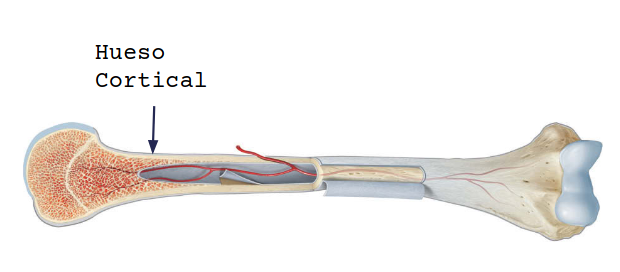
\includegraphics[width=0.75\textwidth]{imagenes/humero.png}
    \caption{Húmero parcialmente seccionado.}
    \label{fig:humero}
\end{figure}


\paragraph{Porosidad Cortical:}
La porosidad cortical consiste en una red de canales que proporcionan conductos para que la vasculatura impregne la corteza y, en última instancia, sostener a los osteocitos
\cite{Cooper2016}.
En la Figura \ref{fig:porosidad}, se muestra un detalle de hueso cortical indicando los canales de la porosidad cortical.

\begin{figure}[H]
    \centering
    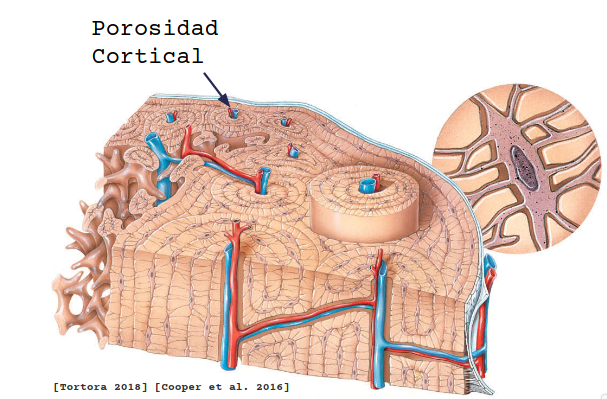
\includegraphics[width=0.75\textwidth]{imagenes/porosidad.png}
    \caption{Vista ampliada de hueso cortical.}
    \label{fig:porosidad}
\end{figure}


\paragraph{Osteocitos:}
Los osteocitos son células oseas maduras, que son las principales del hueso y mantienen su metabolismo diario a través del intercambio de nutrientes y productos metabólicos con la sangre
\cite{tortora/derrickson2018}.

\paragraph{Densidad Mineral Osea:}
La densidad mineral osea (DMO) es la cantidad de materia mineral en el tejido oseo. Las mediciones de densidad osea son usadas en la medicina clínica como un indicador indirecto de osteoporosis y riesgo de fractura
\footnote{https://meshb.nlm.nih.gov/record/ui?ui=D015519}.
En la Figura \ref{fig:bmd}, se muestra una imagen de Densitometría ósea, donde el nivel de gris indica la cantidad de material mineral en el hueso.

\begin{figure}[H]
    \centering
    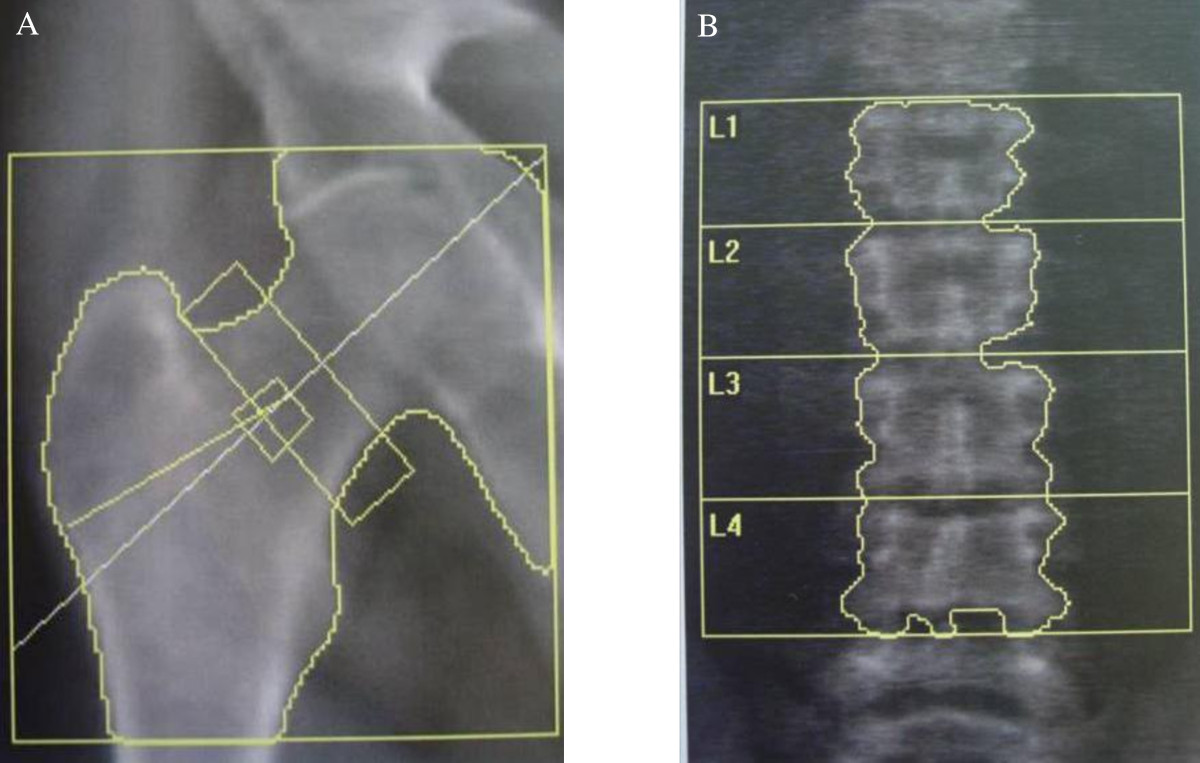
\includegraphics[width=0.75\textwidth]{imagenes/image6.jpg}
    \caption{Imagen de Densitometría ósea.}
    \label{fig:bmd}
\end{figure}

\subsection{Ámbito Ultrasonido}

\paragraph{Ultrasonido:}
El ultrasonido es una onda mecánica con una frecuencia para uso clínico entre 1 y 15 MHz, estas frecuencias son mayores al limite superior audible por un humano (20 KHz). La longitud de onda del ultrasonido en los tejido es entre ~0.1 y 1.5 mm
\cite{nadinebarriesmith2010}
\cite{Abu-Zidan2011}.

\paragraph{Guía de Onda:}
Es una estructura que guía ondas, como las electromagnéticas o mecánicas, con una pérdida mínima de energía al restringir la expansión a una o dos dimensiones.

\paragraph{Transductor de Ultrasonido:}
Son un tipo de sensor acústico, se pueden categorizar como Emisores que convierten señales eléctricas en ultrasonido y como Receptores que convierten el ultrasonido en señales eléctricas
\cite{nakamura2012ultrasonic}.

\paragraph{Placa Libre:}
Una placa es un elemento estructural con dimensiones planas (largo y ancho) son grandes en comparación con su grosor y está sujeto a cargas que causan deformación por flexión además del estiramiento.
En la mayoría de los casos, el grosor no es mayor que una décima parte de la dimensión más pequeña en el plano.
Por libre se asume que la placa no experimenta momentos de flexión y torsión y no hay fuerzas de corte verticales
\cite{ensminger2008ultrasonics}.

\subsection{Ámbito Procesamiento de Señales}

\paragraph{Procesamiento Digital de Señales:}
El procesamiento digital de señales es el uso del procesamiento digital, por ejemplo, en computadoras o procesadores de señales digitales más especializados, para realizar una amplia variedad de operaciones de procesamiento de la señal.
Las señales procesadas de esta manera son una secuencia de números que representan muestras de una variable continua en un dominio como el tiempo, el espacio o la frecuencia.

\paragraph{Transformada de Fourier:}
La Transformada de Fourier toma una función definida en el dominio del tiempo o espacio y la transforma al dominio de la frecuencia, que provee un ambiente natural para el estudio de muchos problemas.
Las técnicas del Análisis de Fourier son usadas en distintos y diversos campos como, por ejemplo el procesamiento de señales, astronomía, geodésica,las imágenes medicas y el análisis de voz
\cite{neilsalkind2006}.
La Figura \ref{fig:tf}, muestra una función y su transformada de Fourier.

\begin{figure}[H]
    \centering
    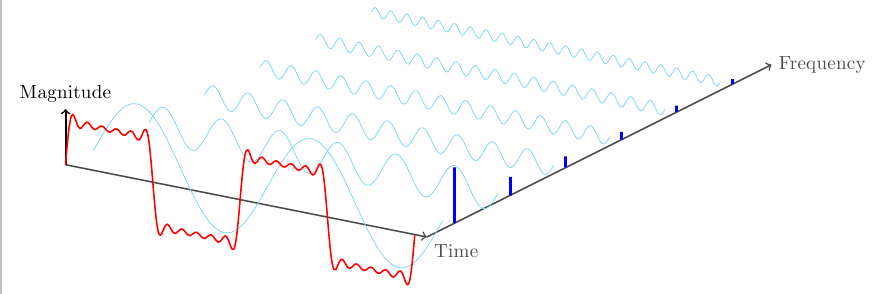
\includegraphics[width=0.75\textwidth]{imagenes/image17.png}
    \caption{Imagen Transformada de Fourier.}
    \label{fig:tf}
\end{figure}


\paragraph{Señal:}
Una señal es una función de uno o más variables independientes, que contienen información sobre el comportamiento o la naturaleza de algún fenómeno
\cite{alanoppenheim2015}.

\paragraph{Descomposición en valores singulares:}
La descomposición de valores singulares (DVS) es una factorización de una matriz $M$ de $m$ filas y $n$ columnas.
Esta factorización tiene la forma $M = U \Sigma V*$, donde $U$ es una matriz cuadrada de orden $m$, donde $\Sigma$ es una matriz diagonal rectangular $n$ x $m$ con valores reales no-negativos en la diagonal y $V$ es una matriz cuadrada de orden $n$.
Los valores de la diagonal de $\Sigma$ son los valores singulares de $M$. Las columnas de $U$ y $V$ son los vectores singulares izquierdos y vectores singulares derechos de $M$ respectivamente.
\cite{leslie2007handbook}

\paragraph{Transmisión Axial:}
La transmisión axial es una técnica de ultrasonido cuantitativa que permite medir el espesor y la porosidad del hueso cortical.
Esta técnica toma en cuenta la capacidad de los huesos largos en guiar onda en el rango de frecuencias (200KHz - 2MHz), que significa la coexistencia  de varios modos guiados.
Usando un sonda compuesta por un arreglo de emisores y receptores dispuestos linealmente, son grabados los modos guiados propagados por el hueso cortical.
La curvas de dispersión se obtienen usando una transformada de Fourier  bidimensional combinada con una descomposición de valores singulares.
Los valores de espesor y porosidad son obtenidos mediante la resolución del problema inverso, donde las curvas de dispersión son predichas desde un modelo de placa libre isotrópica
\cite{Minonzio2018a}.


\section{Estado del Arte}
\label{sc:EA}

El estado de arte para el desarrollo especifico de esta tesis, sera separado en dos áreas, análisis de desempeño y alto rendimiento.

\subsection{Análisis de Desempeño}

\paragraph{Thinking Methodically about Performance}
En este articulo el autor describe dos anti-métodos para el análisis de desempeño, luego señala tres alternativas a las descritas anteriormente y finalmente propone como el uso del Método Utilización, Saturación y Errores (USE) como una mejor alternativa.
El método USE propone la construcción de un \emph{checklist} que sirve para detectar rápidamente cuellos de botella de recursos o errores
\cite{Gregg2013}.
En la Figura \ref{fig:use}, se muestra el diagrama de flujo de la metodología USE.

\begin{figure}[H]
    \centering
    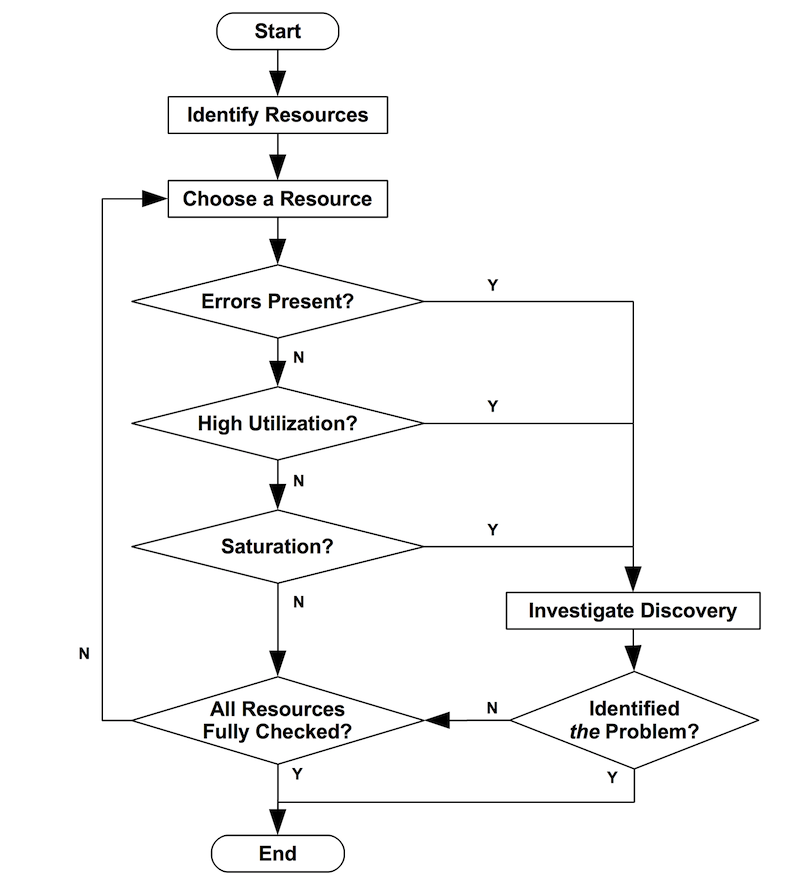
\includegraphics[width=0.75\textwidth]{imagenes/image13.png}
    \caption{Diagrama de flujo de metodología USE.}
    \label{fig:use}
\end{figure}

\paragraph{HPCToolkit - Tools for performance analysis of optimized parallel programs}
Este articulo describe la herramienta HPCTOOLKIT, desarrollada por la Universidad Rice.
HPCToolkit es una suite de herramientas que soporta la medición, análisis, atribución y presentación del desempeño de aplicaciones para programas secuenciales y paralelos.
La metodología en la cual esta basada en un conjunto de principios complementarios
\cite{Adhianto2009}.
A continuación se listan estos principios son:
\begin{itemize}
  \item Ser independiente del lenguaje.
  \item Evitar instrumentación del código.
  \item Evitar puntos ciegos.
  \item El contexto es esencial para entender el software en capas y orientado a objetos.
  \item Cualquier medida de rendimiento por si sola produce una vista miope del problema.
  \item Las métricas de desempeño derivadas son esenciales para un análisis efectivo.
  \item El análisis de rendimiento debe ser de arriba a abajo.
  \item La agregación jerárquica es vital.
  \item La medición y el análisis deben ser escalables.
\end{itemize}
En la Figura \ref{fig:hpctoolkit}, se detallan los principales componentes de HPCToolkit y sus relaciones.

\begin{figure}[H]
    \centering
    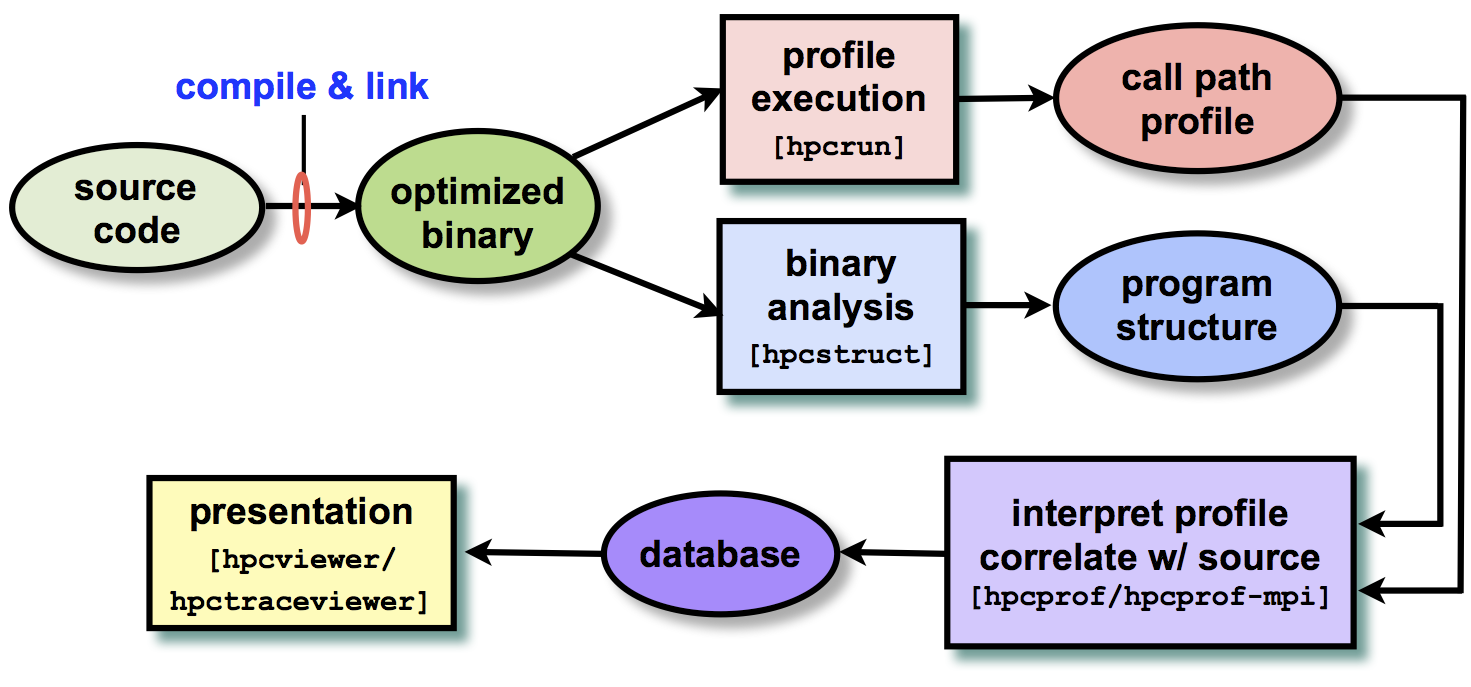
\includegraphics[width=0.75\textwidth]{imagenes/image14.png}
    \caption{Componentes HPCToolkit.}
    \label{fig:hpctoolkit}
\end{figure}



\paragraph{Autoperf - Workflow Support for Performance Experiments}
El articulo presenta la herramienta Autoperf. Esta permite crear y administras experimentos de desempeño, incluyendo el análisis y posprocesamiento de datos
\cite{Dai2015}.
El diseño de la herramienta lo componen cuatro componentes:
\begin{itemize}
  \item Especificación del experimento, este componente es el encargado de entregar la información básica para el experimento e.g., el comando usado para invocar el programa.
  \item Envió del trabajo, encargo de los parámetros que dependen del entorno donde se ejecuta el experimento.
  \item Recolección de datos, Autoperf se basa en las herramientas de rendimiento existentes para recopilar datos de rendimiento.
  Actualmente, TAU y HPCToolkit son compatibles con Autoperf.
  \item Motor de análisis, este modulo es el encargado del análisis estadístico del experimento.
\end{itemize}

\subsection{Alto Rendimiento}

\paragraph{Anatomy of high-performance matrix multiplication}
Los autores en este articulo describen los principios que subyacen en la implementación de una multiplicación de matrices que es usada ampliamente en la librería GotoBlas.
Un desempeño cerca del optimo es obtenido mediante un entendimiento completo de como la operación debe separada en niveles.
La multiplicación de matrices la descompone en distintos casos especiales mas pequeños.
 La idea es si logra alto desempeño en los casos especiales, obtiene alto desempeño en la multiplicación de matrices
\cite{Goto2008}.
En la Figura \ref{fig:hmem}, se muestra modelo simple y refinado de la jerarquía de memoria, estos modelos son necesarios para poder optimizar la multiplicación  de matrices, ya que se analiza el costo de mover datos entre capas de memoria.

\begin{figure}[H]
    \centering
    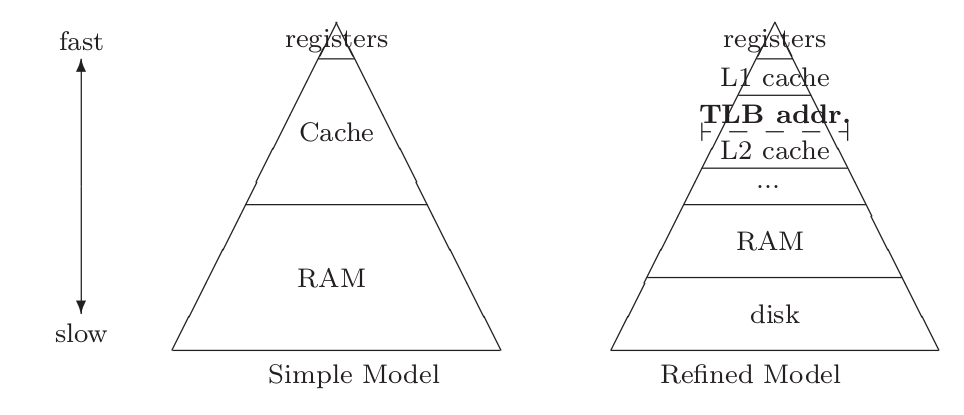
\includegraphics[width=0.75\textwidth]{imagenes/image10.png}
    \caption{Modelos jerárquicos de memoria.}
    \label{fig:hmem}
\end{figure}

\paragraph{High-Performance Matrix-Matrix Multiplications of Very Small Matrices}
El documento describe la falta de librerías especializadas capaces de tener un alto desempeño cuando se dan situaciones donde una aplicación tenga que realizar un calculo que sea acumuladamente grande, pero sus partes individuales sean pequeñas.
Por eso mismo, lo autores desarrollaron algoritmos innovadores, abstracciones de los datos y las tareas y todas la implementaciones basadas en el estándar  MAGMA 2.0
\cite{Masliah2016}


\paragraph{LIBXSMM: Accelerating Small Matrix Multiplications by Runtime Code Generation}
En este articulo se presenta un librería obtiene alto desempeño en la multiplicación de matrices pequeñas.
La aceleración es obtenida usando distintas técnicas. Siendo la mas importante, usar un generador de código con un modelo de arquitectura integrado que crea código que no necesita un fase de \emph{auto-tunning}
\cite{Heinecke2016}.




